\chapter{Simulation Environment}
\section{Introduction}
Small-scale helicopters are highly nonlinear systems with complex coupling. Analyzing velocity fields around the rotor requires complicated experiments and numerical methods, which differ in each flight regime such as hover, stall, etc. \cite{doerffer2008numerical,crittenden2004combustion,patterson1990computational}. There are numerous studies on mathematical models of the helicopter dynamics and governing equations of the forces and moments applied to it \cite{padfield2008helicopter,marques2017advanced, seddon2011basic}. For this study, we have used the model already developed for the Evolution-EX helicopter in \cite{pourrezaei2014control}. Here we briefly discuss the model development of this helicopter.
\section{Governing equations}
A combination of four subsystems describes the Evolution-EX helicopter's (EEH) dynamics: the rigid-body dynamics of the fuselage, the main rotor, the tail rotor, and the empennage. Two frameworks are defined like other dynamic problems: the body (B) and the Inertia (I)  framework. 
\subsection{States and control input}
The states regarding the UAV dynamics include the velocity vector $[3\times1]$:

\begin{equation}
	V=[u,v,w]^T	
\end{equation}

In this equation, u denotes the velocity in the x direction, v represents the velocity in the y direction, and w is the velocity in the z direction.
and the angular velocity vector $[3\times1]$:

\begin{equation}
	\omega=[p,q,r]^T
\end{equation}

In this equation, p represents represent the angular velocity in the p direction, q denotes the angular velocity in the y direction, and r is the angular velocity in the z direction.
with respect to body coordinates {B} and the position vector $[3\times1]$:

\begin{equation}
	p=[x,y,z]^T
\end{equation}

and the Euler angles vector which is roll pitch and yaw $[3\times1]$:

\begin{equation}
	\Theta=[\phi,\theta,\psi]^T
\end{equation}

with respect to inertia framework {I} and the input vector $[4\times1]$:

\begin{equation}
	U=[\delta_{col},\delta_{lat},\delta_{lon},\delta_{ped}]^T
\end{equation} 

the $\delta_{col}$ is the collective input which is responsible for increasing the angle of attack in all the angles of the blade plane, the lateral input $\delta_{lat}$ is responsible to increase the angle of attack for a lateral movement of the helicopter and $\delta_{lon}$ on the other hand is doing the same thing for a longitudinal movement. The $\delta_{ped}$ increases the angle of attack of the blades for the tail rotor in the same way that $\delta_{col}$ does for the main rotor blades.
In the next section the governing equations regarding the states are discussed

\subsection{State-space equations}

The Newton-Euler equations of motion of the helicopter fuselage are defined as:

\begin{equation}\label{eq1}
	\dot{V}=\frac{1}{m} F-\omega\times V
\end{equation}

\begin{equation}\label{eq2}
	\dot{\omega}=I^{-1}M-I^{-1}(\omega \times I \omega) 
\end{equation}

\begin{equation}
	\dot{\Theta}=\Phi(\Theta)\omega 
\end{equation}

\begin{equation}
	\dot{p}=R_{b}^I(\Theta)V
\end{equation}

F and M are defined as vector of external forces and moments respectively. Derivation of F and M are elaborated in \ref{force section} and \ref{Moment section} respectively. $R_b^I$ and $\Phi$ are linear and angular velocity transformation matrices given as follows: 
\begin{gather}
	R_b^I
	=
	\begin{bmatrix}
		s(\theta)c(\psi) &
		-c(\phi)sin(\psi)+s(\phi)s(\theta)c(\psi)&
		s(\phi)s(\psi)+c(\phi)s(\theta)c(\psi) \\
		c(\theta)s(\psi) &
		c(\phi)c(\psi)+s(\phi)s(\theta)s(\psi)&
		-s(\phi)c(\psi)+c(\phi)s(\theta)s(\psi)\\
		-s(\theta)&
		s(\phi)c(\theta)&
		c(\phi)c(\theta)
	\end{bmatrix}
\end{gather}

\begin{gather}
	\Phi
	=
	\begin{bmatrix}
		1 &
		s(\phi)t(\theta)&
		c(\phi)t(\theta) \\
		0 &
		c(\phi)&
		-s(\phi)\\
		0&
		\frac{s(\phi)}{c(\theta)} &
		\frac{c(\phi)}{c(\theta)}
	\end{bmatrix}
\end{gather}

in which s, c and t stands for "sin", "cos" and "tan" respectively.
The I is the moment of inertia in which the off-diagonal terms are neglected:

\begin{equation}
	I=
	\begin{bmatrix}
		I_{xx} &
		0&
		0 \\
		0 &
		I_{yy}&
		0\\
		0&
		0&
		I_{zz}
	\end{bmatrix}
\end{equation}

The $I_{xx}$, $I_{yy}$ and $I_{zz}$ are the rolling, pitching and yawning moment of inertia.\\

In the following sections, equations regarding the derivation of forces and moments in \ref{eq1} and \ref{eq2} are introduced.
\subsection{Blade flapping}

The dynamics of main rotor and stabilizer bar of the EEH is modeled by \textit{hybrid model approach} \cite{mettler2002system}. In this approach $\dot{a}$ and $\dot{b}$ are  tip-path-plane (TPP) longitudinal and lateral flapping angles respectively and the coefficients of first harmonic approximation in the Fourier series form. The rotor flapping state equations are:

\begin{equation}
	\dot{a}=-q-\frac{a}{\tau_{f}}+\frac{1}{\tau_{f}}(K_u\mu_x+K_w\mu_z)+\frac{A_{lon}}{\tau_{f}} (\delta_{lon}+K_c c)+A_b\frac{b}{\tau_{f}}
\end{equation}

\begin{equation}
	\dot{b} = -p-\frac{b}{\tau_{f}}+\frac{1}{\tau_{f}}(K_v\mu_y)+\frac{B_{lat}}{\tau_{f}}(\delta_{lat}+K_d d)+B_a \frac{a}{\tau_{f}}
\end{equation}

$K_u$ is the flapping due to the forward velocity factor, the $K_v$ on the other hands denotes the flapping due to the side-way velocity factor. In the same way, $K_w$ is considered to be te flapping due to downward velocity factor. $K_c$ reflects the longitudinal flapping due to the stabilizer bar factor and $K_d$ depicts the lateral flapping due to the stabilizer bar factor. $A_{lon}$ denotes the longitudinal cyclic to flap gain at nominal rpm and $B_{lat}$ is the lateral cyclic to flap gain at nominal rpm. Last but not least, the $\tau_f$ is the main rotor flapping time-constant.\\
$\mu_x,\mu_y$ and $\mu_z $ are the non-dimensional airflow components defined as:

\begin{equation}
	\begin{aligned}
		\mu_x&=\frac{u-u_{wind}}{\Omega R_{mr}}\\
		\mu_y&=\frac{v-v_{wind}}{\Omega R_{mr}} \\
		\mu_z&= \frac{w-w_{wind}}{\Omega R_{mr}}\\
	\end{aligned}
\end{equation}

And the $K_{u}$, $K_v$ and $K_w$ are given by:

\begin{equation}
	K_{u}=2K_{\mu}(\frac{4}{3}\delta_{col}-\frac{Vi}{\omega R_{mr}})
\end{equation}

\begin{equation}
	K_v=-K_u
\end{equation}

\begin{equation}
	K_w=16K_{\mu} \mu_{mr}^2 \frac{sign(\mu_{mr})}{(1-\mu_{mr}^2/2)*(8sign(\mu_{mr})+CL_\alpha \sigma)}
\end{equation}

The stabilizer bar state equations c and d are TPP longitudinal and lateral flapping angles of the stabilizer bar given by:

\begin{equation}
	\dot{c}=-q-\frac{c}{\tau_s}+\frac{C_{lon}}{\tau_s}\delta_{lon}
\end{equation}

\begin{equation}
	\dot{d}=-p-\frac{d}{\tau_s}+\frac{D_{lat}}{\tau_s}\delta_{lat}
\end{equation} 

\subsection{Force derivation} \label{force section}
 \tikzset{
	every label/.append style={font=\scriptsize},
	my edge labels/.style={font=\scriptsize},
	dominant/.append style={label=below:$dominant$},
}


The force is derived as follows:

\begin{equation}
	F= 
	\begin{bmatrix}
		F_x \\
		F_y\\
		F_z\\
	\end{bmatrix}
	+R_b^I \begin{bmatrix}
		0 \\
		0\\
		mg\\
	\end{bmatrix}
\end{equation}

in which $F_x$, $F_y$ and $F_z$ are defined as:

\begin{equation}
	F_x=-a\ T_{mr}+F_{x,fus}
\end{equation}

\begin{equation}
	F_y=b\ T_{mr}+T_{tr}+F_{y,fus} + F_{y,vt}
\end{equation}

\begin{equation}
	F_z=-T_{mr}+F_{z,fus} + F_{z,ht}
\end{equation}

$T_{mr}$ is the main rotor thrust and $T_{tr}$ denotes the tail rotor thrust. $T_{mr}$ is given by:

\begin{equation}
	T_{mr} = \textbf{f}_{T_{mr}}+\textbf{b}_{T_{mr}}U;
	\label{T_mr}
\end{equation}

in which $\textbf{f}_{T_{mr}}$ is the autonomous term of the main rotor thrust:

\begin{equation}\label{f_t}
	\textbf{f}_{T_{mr}}= \frac{1}{4} \rho \pi R_{mr}^4\Omega^2\sigma_{mr}(C_{L_{0}}(\frac{2}{3}+\mu_x^2+\mu_y^2)+C_{L_{\alpha}}(\mu_z-\lambda_0))
\end{equation}

In which $R_{mr}$ is the main rotor radius and $\Omega$ represents the nominal main rotor speed. $\sigma_{mr}$ depicts the main rotor solidity factor and $C_{L0}$ and $C_{L\alpha}$ are the main rotor blade zero lift curve and blade lift curve slope respectively.\\
$\lambda_0$ is the inflow ratio expressed as:

\begin{equation}
	\lambda_0=\frac{V_i}{\Omega R_{mr}}
\end{equation}

The solidity factor derived by:

\begin{equation}
	\sigma_{mr}=\frac{Nc_{mr}}{\pi R_{mr}}
\end{equation}

and $b_{T_{mr}}$ in \ref{T_mr} is control input coefficient term given by:

\begin{equation}\label{b_T}
	\textbf{b}_{T_{mr}}= \frac{1}{4} \rho \pi R_{mr}^4 \Omega^2 \sigma_{mr} C_{L_{\alpha}}\begin{bmatrix}
		\mu_x^2+\mu_y^2+\frac{2}{3}&
		-\mu_y&
		\mu_x&
		0
	\end{bmatrix}
\end{equation}

Similarly, it is possible to derive the tail rotor thrust $T_{tr}$:

\begin{equation}
	T_{tr} = \textbf{f}_{T_{tr}}+\textbf{b}_{T_{tr}}U;
\end{equation}

In which $\textbf{f}_{T_{tr}}$ is the autonomous term of the tail rotor thrust:

\begin{equation}\label{f_t_tr}
	\textbf{f}_{T_{tr}}=- \frac{1}{4} \rho \pi R_{tr}^4 n_{tr}^2\Omega^2\sigma_{tr}C_{L\alpha_{tr}}v_{tail}
\end{equation}

And input coefficients $b_{T_{tr}}$ is given by:

\begin{equation}\label{b_Ttr}
	\textbf{b}_{T_{tr}}= -\frac{1}{4} \rho \pi R_{tr}^4 n_{tr}^2 \Omega^2 \sigma_{tr} C_{L\alpha_{tr}}\begin{bmatrix}
		0&
		0&
		0&
		u_{tail}^2+w_{tail}^2+\frac{2}{3}
	\end{bmatrix}
\end{equation}

The normalized velocities at tail rotor can be given as:

\begin{equation}
	\begin{aligned}
		u_{tail}&=\frac{u-u_{wind}}{\Omega_{tr} R_{tr} }\\
		v_{tail}&=\frac{v-v_{wind}-V_{i_{tr}}+x_{fus}r}{\Omega_{tr} R_{tr}} \\
		w_{tail}&= \frac{w-w_{wind}-K_{\lambda}V_i+x_{fus}q}{\Omega_{tr} R_{tr}}\\
	\end{aligned}
\end{equation}

The tail rotor nominal speed is given by:

\begin{equation}
			\Omega_{tr}=n_{tr}\Omega  
\end{equation}

In which the $n_{tr}$ is gear ratio of tail rotor to main rotor. $F_{y,vt}$ is the vertical tail force derived by:

\begin{equation}\label{Yvt}
	F_{y,vt}=\frac{1}{2} \rho S_{vt} \Big( C_{L_\alpha}^{vt}V_{vt}(v-v_{wind})+v_{tail}^2 \Big)
\end{equation}

In the above equation, the $\rho$ is the air density. $S_{vt}$ denotes the vertical tail area, 
And horizontal tail force $F_{z,ht}$ is:

\begin{equation} \label{Z_ht}
	F_{z,ht}=\frac{1}{2} S_{ht} \Big( C_{L_{\alpha}}^{ht} \mid u-u_{wind} \mid w_{ht} +w_{ht}^2 \Big)    
\end{equation}

In equation \ref{Yvt} $V_{vt}$ and $v_{tail}$ are axial and normal velocities in vertical tale defined as:

\begin{equation}
	\begin{aligned}
		V_{vt}&=\sqrt{(u-u_{wind})^2+(w- w_{wind} +x_{vt}q-K_\lambda V_i)^2}\\
		v_{tail}&=v-v_{wind}+x_{vt}r-V_{i_{tr}} \\
	\end{aligned}
\end{equation}

Similarly in equation $w_{ht}$ is the horizontal tail velocity in the z direction \ref{Z_ht}:

\begin{equation}
	w_{ht}=w-w_{wind}-x_{ht}q-K_{\lambda}V_i
\end{equation} 

The $K_{\lambda}$ is the main rotor downwash factor at fuselage.\\

$F_{z,fus} , F_{y,fus}$ and $F_{x,fus}$ are drag forces derived by:

\begin{equation}
	F_{x,fus}=-\frac{1}{2} \rho S_x^{fus} V_{fus} (u-u_{wind})
	\label{X_fus}
\end{equation}

\begin{equation}\label{Y_fus}
	F_{y,fus}=-\frac{1}{2} \rho S_y^{fus} V_{fus} (v-v_{wind})
\end{equation}

\begin{equation}\label{Z_fus}
	F_{z,fus}=-\frac{1}{2} \rho S_z^{fus} V_{fus} (w-w_{wind}+V_i)
\end{equation}

the dynamic pressure of the fuselage $V_{fus}$ in expression \ref{X_fus} is defined as:

\begin{equation}
	V_{fus}=\sqrt{(u-u_{wind})^2+(v-v_{wind})^2+(w-w_{wind}+V_i)^2}
\end{equation}

\subsection{Moment derivation} \label{Moment section}

Moment includes 3 terms roll, pitch and yaw:

\begin{equation}
	M =\begin{bmatrix}
		M_{roll}\\
		M_{pitch}\\
		M_{yaw}\\
	\end{bmatrix}
\end{equation}

The three terms in the above equation are given as:

\begin{equation}
	M_{roll} = (K_{\beta}-T_{mr}Z_{cg})b;%-Ttail*z_fus;
\end{equation}

\begin{equation}
	M_{pitch} = (K_\beta-T_{mr}Z_{cg})a;
\end{equation}

\begin{equation}
	M_{yaw} = Q_{mr}+T_{tr}x_{fus};
\end{equation}

$Z_{cg}$ is the Main rotor hub height from center of gravity and $x_{fus}$ is the tail rotor hub offset from center of gravity along x-axis.
Main rotor drag torque $Q_{mr}$ is derived by:
\begin{equation}
	Q_{mr} = \textbf{f}_{Q_{mr}}+\textbf{b}_{Q_{mr}}U;
\end{equation}
In which the main rotor drag torque terms are given as:
\begin{equation} \label{f_Q}
	\textbf{f}_{Q_{mr}}=\frac{1}{8} \rho \pi R_{mr}^5 \Omega^2 \sigma_{mr} C_{L_{\alpha}}  \bigg( \frac{C_{D0}}{C_{L_{\alpha}}} \Big( \mu_x^2+\mu_y^2+1 \Big)-2(\mu_{z}-\lambda_0)^2 \bigg)
\end{equation}
\begin{equation} \label{b_Q}
	\textbf{b}_{Q_{mr}}=\frac{1}{8} \rho \pi R_{mr}^5 \Omega^2 \sigma_{mr} C_{L_{\alpha}} (\lambda_0-\mu_z)  \begin{bmatrix}
		\frac{4}{3}
		-\mu_y&
		\mu_x &
		0
	\end{bmatrix}  
\end{equation}

\subsection{Induced velocity}

As indicated in \cite{johnson2012helicopter} and \cite{leishman2006principles} the blade element analysis considers each blade
element as a two-dimensional airfoil. The aerodynamic behavior of neighboring
blade elements is independent of each other. An induced inflow velocity on each
blade element should be accounted for, which is a product of the rotor wake. Analytical
ways of calculating the induced velocity may be found using momentum theory,
vortex theory, or nonuniform inflow calculations \cite{johnson2012helicopter}.\\

In general, the inflow velocity calculation is a challenging task due to its non-uniformity across the blade span; mathematical simplifications should be applied to minimize the complexity of the analysis. Finally, after determining the velocity components
of the blade element, the aerodynamic forces acting on this element are calculated.
The complete dynamic behavior of the blade is obtained by integrating the applied
forces of the individual elements throughout the blade span. Here we use an experimental approach for induced velocity. \\

$V_i$ and $V_{i_{tr}}$ are induced velocity in main rotor and tail rotor respectively. $V_i$ is given by:

\begin{equation}
	V_i=\frac{v_a}{\sqrt{1+\bar{\mu}^2}}
\end{equation}

In which:

\begin{equation}
	V_h=\sqrt{mg/(2\rho \pi R_{mr}^2)}
\end{equation}

\begin{equation}
	\mu=\sqrt{\mu_x^2+\mu_y^2} 
\end{equation}

\begin{equation}
	\bar{\mu}=\frac{\mu}{V_h/(\Omega R_{mr})} 
\end{equation}

\begin{equation}
	V_a=-\frac{w-w_{wind}}{V_h}
\end{equation}

\begin{equation}
	v_a = \left\{
	\begin{array}{ll}
		-\frac{1}{2} V_a-\sqrt{\frac{V_a^2}{4}-1} & \mbox{if } \ V_a 	\leqslant -2 \\
		1-\frac{1}{2} V_a+\frac{25}{12} V_a^2 +\frac{7}{6} V_a^3 & \mbox{if } \ -2<V_a<0 \\
		-\frac{1}{2} V_a+\sqrt{\frac{V_a^2}{4}+1} & \mbox{if } \ V_a	\geqslant 0 \\
	\end{array}
	\right.
	\label{vamr}
\end{equation}

Similarly, $V_{i_{tr}}$ is:

\begin{equation}
	V_{i_{tr}}=\frac{v_{a_{tr}}}{\sqrt{1+\overline{\mu_{tr}}^2}}
\end{equation}

In which:

\begin{equation}
	V_{h_{tr}}=\sqrt{f_{F_{y,mr}}/(2\rho \pi R_{tr}^2 x_{fus} )}
\end{equation}

\begin{equation}
	\mu_{tr}=\sqrt{u_{tail}^2+w_{tail}^2} 
\end{equation}

The $\overline{\mu}_{tr}$ is the advance ratio normalized by $V_{h_{tr}}/(\Omega R_{tr}$:

\begin{equation}
	\overline{\mu}_{tr}=\frac{\mu_{tr}}{V_{h_{tr}}/(\Omega R_{tr})} 
\end{equation}

\begin{equation}
	V_{a_{tr}}=-\frac{v-v_{wind}+x_{fus}r}{V_h}
\end{equation}

\begin{equation}
	v_{a_{tr}} = \left\{
	\begin{array}{ll}
		-\frac{1}{2} V_{a_{tr}}-\sqrt{\frac{V_{a_{tr}}^2}{4}-1} & \mbox{if } \ V_{a_{tr}} 	\leqslant -2 \\
		1-\frac{1}{2} V_{a_{tr}}+\frac{25}{12} V_{a_{tr}}^2 +\frac{7}{6} V_{a_{tr}}^3 & \mbox{if } \ -2<V_{a_{tr}}<0 \\
		-\frac{1}{2} V_{a_{tr}}+\sqrt{\frac{V_{a_{tr}}^2}{4}+1} & \mbox{if } \ V_{a_{tr}}	\geqslant 0 \\
	\end{array}
	\right.
	\label{vatr}
\end{equation}

Instead of using equation \ref{vamr} and \ref{vatr}, we use the following approximate functions by regression as they provide a faster calculation time in simulations:

\begin{equation}
	v'_a = \frac{4.055}{{\left(1.28V_{a}+1.45\right)}^2+1.7}+0.066
\end{equation}

\begin{equation}
	v'_{a_{tr}} = \frac{4.055}{{\left(1.28V_{a_{tr}}+1.45\right)}^2+1.7}+0.066
\end{equation}

Figure \ref{fig_va} depicts the two functions $v_a$ and $v'_a$ based on $V_a$.

\begin{figure}
	\begin{center}
		{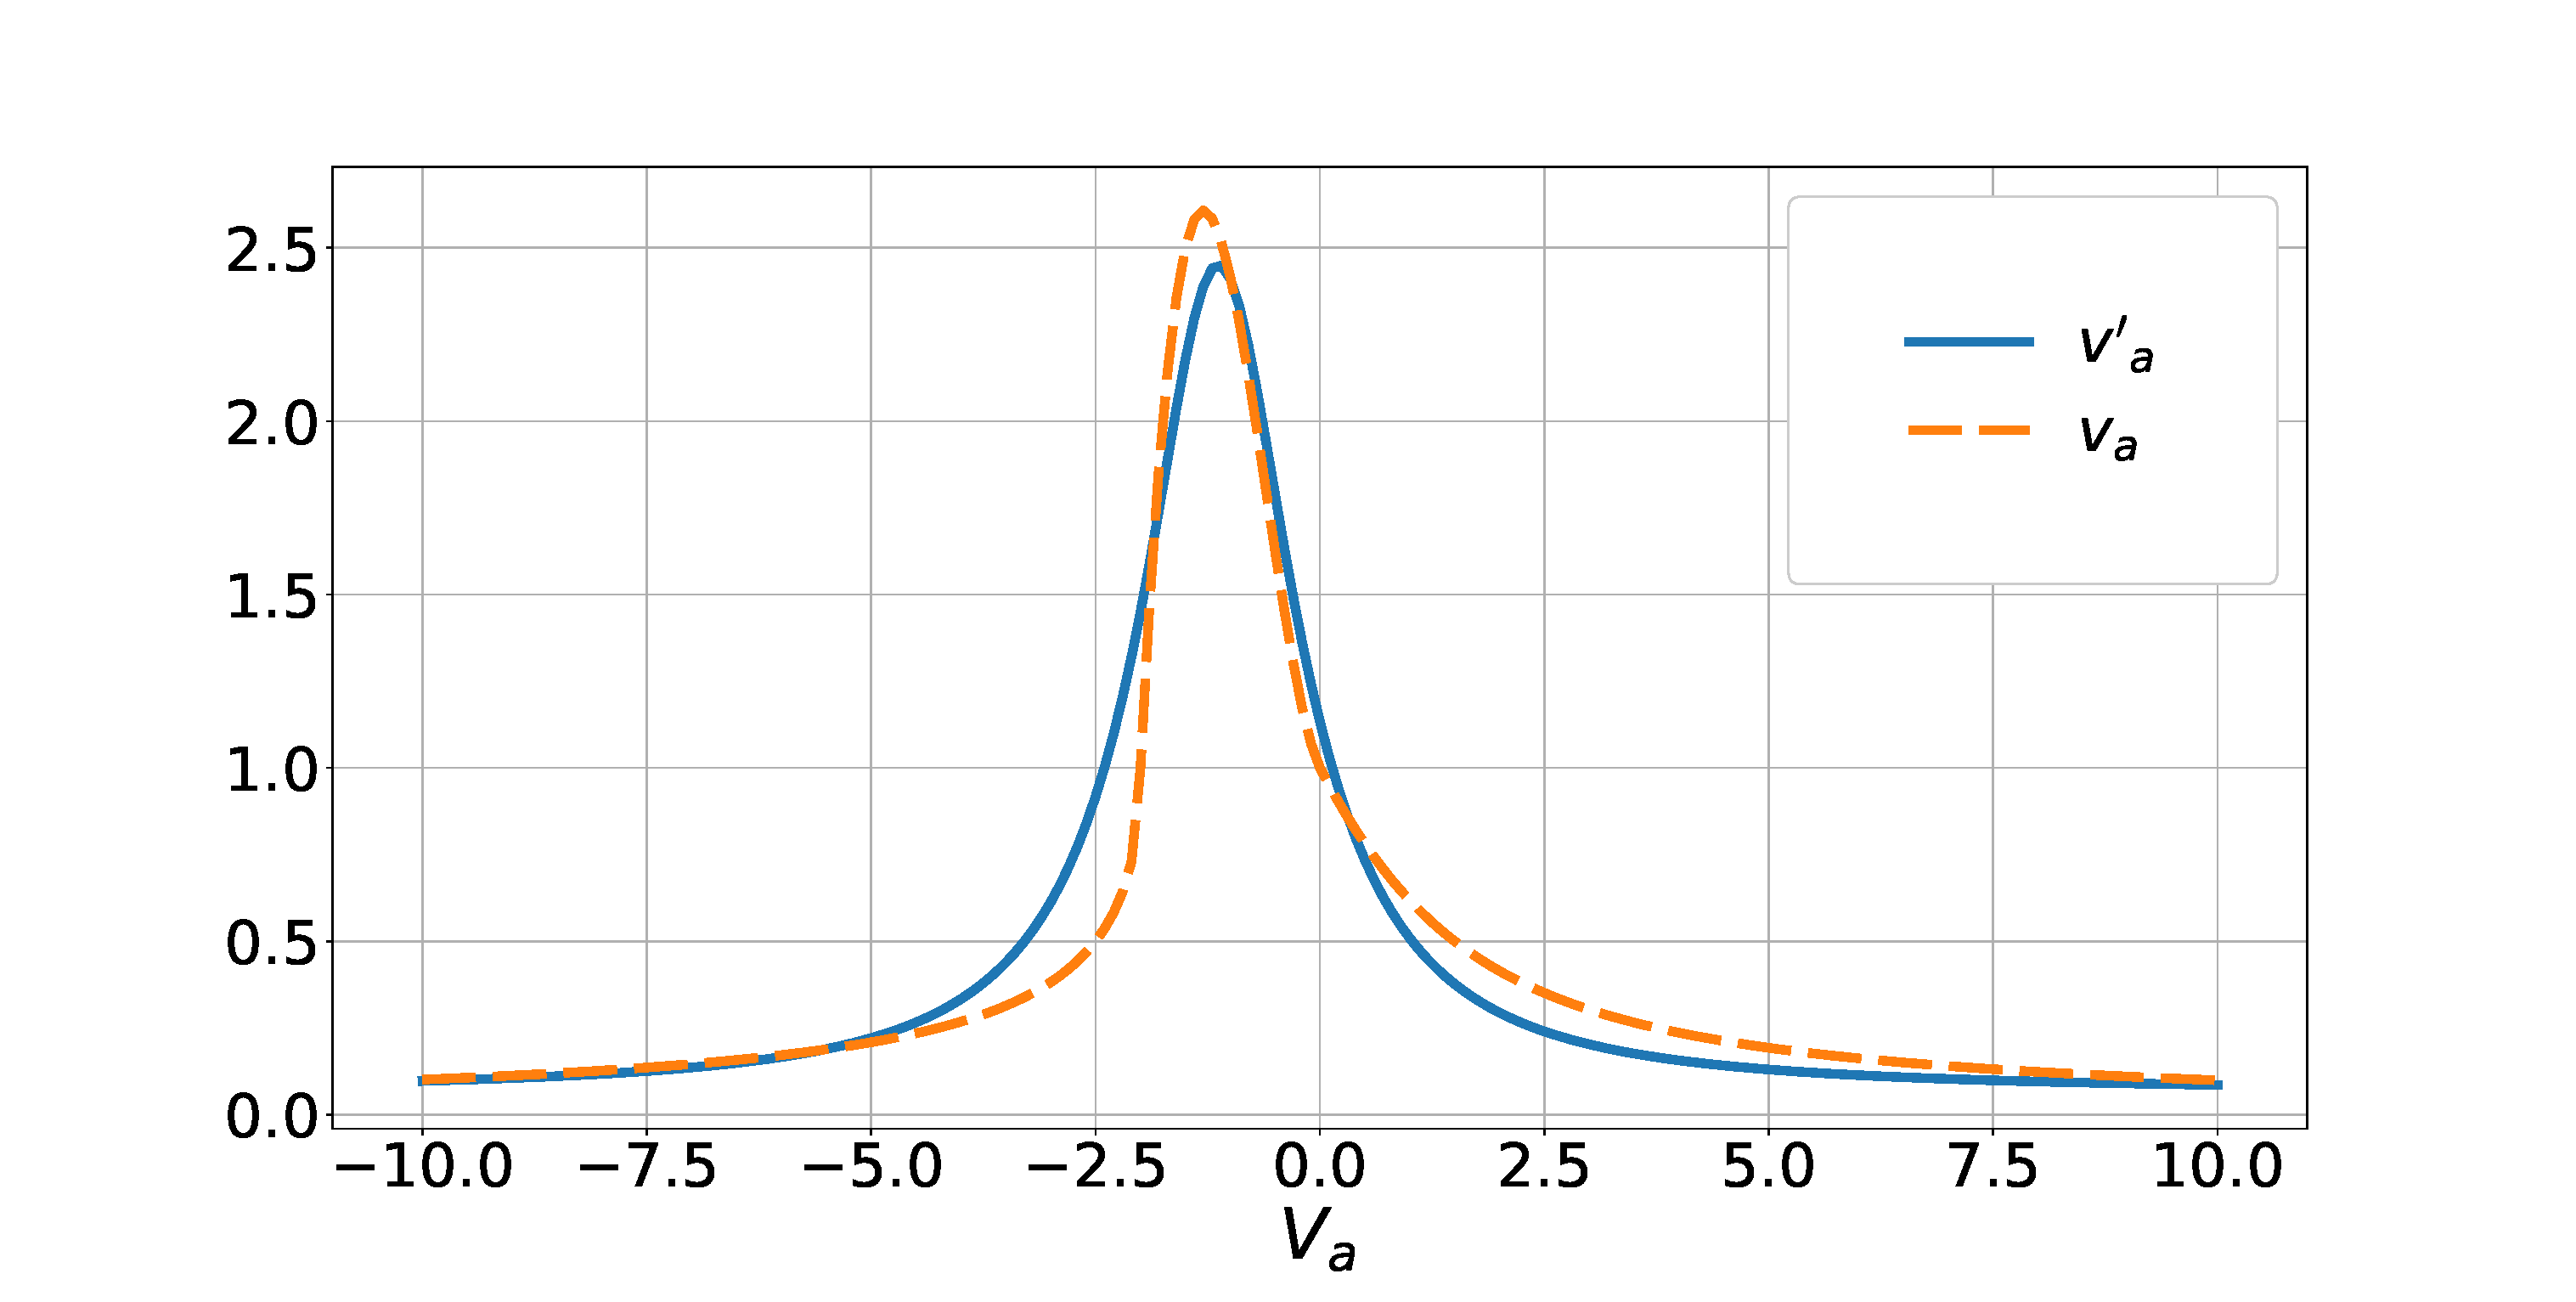
\includegraphics[scale=0.3]{va.eps}}
		
		\caption{Function approximation of $v_a$ by $v'_a$, $R^2=0.947$.}
		\label{fig_va}
	\end{center}
\end{figure}

The constant parameters in the above modeling is given in the table \ref{helicopter_parameters}.
\begin{longtable}{c|c|c||c|c|c} 
	\caption {Constant parameters in the helicopter modeling}\label{helicopter_parameters}\\\toprule
	\endfirsthead
	\caption* {\textbf{Table \ref{helicopter_parameters} Continued:} }\\\toprule
	\endhead
	\endfoot
	\bottomrule
	\endlastfoot
	\textbf{Parameter} & \textbf{Value} & \textbf{Dimension} & \textbf{Parameter} & \textbf{Value} & \textbf{Dimension} \\ \hline \hline
	$\alpha_{1}$ & $53$ &  $[-]$ & $\alpha_{2}$ & $55$ &  $[-]$ \\  \hline
	$ \Omega$ & $115 $ &  $[rad/s]$ & $\rho $ & $1.107 $ &  $[kg/m^3]$ \\ \hline
	$ \tau_f$ & $0.04 $ &  $[s]$ & $\tau_s $ & $ 0.2$ &  $[s]$ \\ \hline
	$\tau_s $ & $ 0.2$ &  $[s]$ & $A_b $ & $-0.1 $ &  $ [-]$ \\ \hline
	$A_{lon} $ & $ 1$ &  $[-]$ & $B_a $ & $0.1 $ &  $ [-]$ \\ \hline
	$B_{lat} $ & $0.9875 $ &  $[-]$ &$C_{D0_{tr}} $ & $0.06 $ &  $[-]$  \\ \hline
	$C_{D0} $ & $0.01 $ &  $[-]$ & $C_{L0} $ & $0.008 $ &  $[-]$ \\ \hline
	$C_{L\alpha_{tr}} $ & $4.95 $ &  $[rad^{-1}]$ & $C_{L\alpha} $ & $5.49 $ &  $[rad^{-1}]$ \\ \hline
	$c_{mr} $ & $0.082 $ &  $[m]$ & $c_{tr} $ & $0.025 $ &  $[m]$ \\ \hline
	$I_{xx} $ & $ 0.3$ &  $[kg.m^2] $  & $I_{yy}$ & $1.6$ & $[kg.m^2]$ \\ \hline
	$I_{zz} $ & $2.0 $ &  $[kg.m^2]$ & $K_\lambda $ & $1 $ &  $[-] $ \\ \hline
	$K_s $ & $0.3 $ &  $[-] $  & $K_\beta $ & $ 255$ &  $[N.m]$ \\ \hline
	$K_{lat} $ & $0.98 $ &  $[-] $  & $K_{lon} $ & $1 $ &  $[-] $ \\ \hline
	$m $ & $11.5 $ &  $[kg] $  & $n_{tr} $ & $6 $ &  $[-] $ \\ \hline
	$R_{mr} $ & $0.95 $ &  $[m]$  & $R_{tr} $ & $0.15 $ &  $[m] $ \\ \hline
	$S_x^{fus} $ & $0.1 $ &  $[m^2] $  & $S_y^{fus} $ & $0.83 $ &  $[m^2] $ \\ \hline
	$S_z^{fus} $ & $0.51 $ &  $[m^2] $  & $x_{fus} $ & $-1.22 $ &  $[m] $ \\ \hline
	$z_{CG}$ & $-0.32 $ &  $[m] $  &  &  & \\ 
\end{longtable}

\section{Sliding mode control}
In order to compare the results obtained by the RL method to a traditional control method, we here provide the details of a sliding mode controller as a nonlinear method. As it is an under actuated system which means that there are only have 4 inputs and 6 states to control. Based on \cite{slotine1991applied,pourrezaei2014control} in order to use sliding mode controller on a helicopter, first we have to change it to a square and affine in control form  so  we discuss how this is achieved.

\subsection{Force derivation in control affine form} \label{force section_affine}
In order to provide a control input by sliding mode controller, each of the force and moment should be linearized based on the control input. Control-affine form of each term is given as a input coefficient "b" and a "f" term which is related to autonomous response of the system. Force is given as:

\begin{equation}\label{Force eq}
	F=\textbf{f}_F+\textbf{b}_FU
\end{equation}

$f_F$ is the autonomous term of the force expressed as:
\begin{gather}\label{F_0}
	\textbf{f}_F
	=
	\begin{bmatrix}
		\textbf{f}_{F_{x,mr}}+F_{x,fus} \\
		\textbf{f}_{F_{y,mr}}+\textbf{f}_{F_{y,tr}}+F_{y,vt}+F_{y,fus}\\
		\textbf{f}_{F_{z,mr}}+F_{z,ht}+F_{z,fus} \\
	\end{bmatrix}
	+R_b^{I^{-1}}\begin{bmatrix}
		0 \\
		0\\
		mg \\
	\end{bmatrix}
\end{gather}

in which:

\begin{equation}\label{f_X_MR}
	\textbf{f}_{F_{x,mr}}=\textbf{f}_T(\tau_f q-a_v)
\end{equation}
 
\begin{equation}
	F_{x,fus}=-\frac{1}{2} \rho S_x^{fus} V_{fus} (u-u_{wind})
	\label{X_fus}
\end{equation}

\begin{gather}\label{f_Y_MR}
	\textbf{f}_{F_{y,mr}}=(\tau_fp+b_v)\textbf{f}_T
\end{gather}

\begin{equation}
	\textbf{f}_{F_{y,tr}}=\textbf{f}_{T_{tr}} 
\end{equation}



\begin{equation}
	\textbf{f}_{F_{z,mr}}=-\textbf{f}_T    
\end{equation}


$a_v$ and $b_v$ in \ref{f_X_MR} and \ref{f_Y_MR} are respectively longitudinal and lateral translational velocity contributions to the flapping of the main rotor  and defined by the following terms:

\begin{equation}
	\begin{aligned}
		a_v&=\frac{\partial a_1}{\partial \mu_x} \mu_x+\frac{\partial a_1}{\partial \mu_z} \mu_z \\
		b_v&=\frac{\partial a_1}{\partial \mu_y}\mu_y 
	\end{aligned}
\end{equation}

the dynamic pressure of the fuselage in expression \ref{X_fus} is defined as:

\begin{equation}
	V_{fus}=\sqrt{(u-u_{wind})^2+(v-v_{wind})^2+(w-w_{wind}+V_i)^2}
\end{equation}



$\textbf{f}_{T_{mr}}$ is the main rotor thrust autonomous term in the control affine form given by \ref{f_t}.
and $\lambda_0$ is the inflow ratio expressed as:

\begin{equation}
	\lambda_0=\frac{V_i}{\Omega R_{mr}}
\end{equation}

$\sigma_{mr}$ is the solidity factor derived by:

\begin{equation}
	\sigma_{mr}=\frac{Nc_{mr}}{\pi R_{mr}}
\end{equation}

The velocities at tail rotor can be normalized given as:

\begin{equation}
	\begin{aligned}
		u_{tail}&=\frac{u-u_{wind}}{\Omega_{tr} R_{tr} }\\
		v_{tail}&=\frac{v-v_{wind}-V_{i_{tr}}+x_{fus}r}{\Omega_{tr} R_{tr}} \\
		w_{tail}&= \frac{w-w_{wind}-K_{\lambda}V_i+x_{fus}q}{\Omega_{tr} R_{tr}}\\
		\Omega_{tr}&=n_{tr}\Omega  
	\end{aligned}
\end{equation}

similarly velocities at vertical tail or horizontal tail can be defined.\\ 
In equation \ref{Yvt} $V_vt$ and $v_{tail}$ are axial and normal velocities in vertical tale defined as:

\begin{equation}
	\begin{aligned}
		V_{vt}&=\sqrt{(u-u_{wind})^2+(w- w_{wind} +x_{vt}q-K_\lambda V_i)^2}\\
		v_{tail}&=v-v_{wind}+x_{vt}r-V_{i_{tr}} \\
	\end{aligned}
\end{equation}

Similarly in equation \ref{Z_ht}:

\begin{equation}
	w_{ht}=w-w_{wind}-x_{ht}q-K_{\lambda}V_i
\end{equation} 

$b_F$ in equation \ref{Force eq} is the input coefficient of the force which is defined as:

\begin{gather}\label{F_U}
	\textbf{b}_F
	=
	\begin{bmatrix}
		\textbf{b}_{F_{x,mr}}\\
		\textbf{b}_{F_{y,mr}}+\textbf{b}_{F_{y,tr}}\\
		\textbf{b}_{F_{z,mr}}\\
	\end{bmatrix}
\end{gather}

In which the following terms are used:

\begin{equation}
	\textbf{b}_{F_{x,mr}}=(\tau_f q-a_v)\textbf{b}_T-\begin{bmatrix}
		0&0&K_{lon}\textbf{f}_T&0
	\end{bmatrix}
\end{equation}

\begin{gather}
	\textbf{b}_{F_{y,mr}}=(-\tau_fp+b_v)\textbf{b}_T- \begin{bmatrix}
		0&K_{lat}\textbf{f}_T&0&0
	\end{bmatrix}
\end{gather}

\begin{equation}
	\textbf{b}_{F_{y,tr}}=\textbf{b}_{T_{tr}} 
\end{equation}

\begin{equation}
	\textbf{b}_{ F_{z,mr}}=-\textbf{b}_T
\end{equation}

$b_T$ and $b_{T_{tr}}$ is the main rotor thrust input coefficient in the control affine form given as \ref{b_T} and \ref{b_Ttr}.

\subsection{Moment derivation in control affine form} \label{Moment section_affine}
Control affine form of moment is given as:

\begin{equation} \label{M}
	M=\textbf{f}_M+\textbf{b}_M U
\end{equation}

$\textbf{f}_M$ is calculated by:

\begin{gather}\label{M_0}
	\textbf{f}_M
	=
	\begin{bmatrix}
		\textbf{f}_{ M_{x,mr}}+\textbf{f}_{ M_{x,tr}}+ M_{x,vt} \\
		\textbf{f}_{ M_{y,mr}}+\textbf{f}_{ M_{y,tr}}+ M_{y,ht}\\
		\textbf{f}_{ M_{z,mr}}+\textbf{f}_{ M_{z,tr}}+ M_{z,vt} \\
	\end{bmatrix}
\end{gather}

in which:

\begin{equation}
	\textbf{f}_{ M_{x,mr}}=(-\tau_fp+b_v)(K_{\beta}-\textbf{f}_T*z_{cg})
\end{equation}

\begin{equation}
	\textbf{f}_{ M_{x,tr}}=-z_{fus}\textbf{f}_{T_{tr}}
\end{equation}

\begin{equation}
	M_{x,vt}=-F_{y,vt}z_{vt}
\end{equation}

\begin{equation}
	\textbf{f}_{ M_{y,mr}}=(-\tau_fq+a_v)(K_{\beta}-\textbf{f}_T z_{cg})
\end{equation}

\begin{equation}\label{f_M_TR}
	\textbf{f}_{ M_{y,tr}}=\textbf{f}_{Q_{tr}}
\end{equation}

\begin{equation}
	M_{y,ht}=- F_{z,ht}x_{ht}
\end{equation}
 
\begin{equation} \label{f_N_MR}
	\textbf{f}_{ M_{z,mr}}=\textbf{f}_Q
\end{equation}

\begin{equation}
	\textbf{f}_{ M_{z,tr}}=x_{fus}\textbf{f}_{T_{tr}}
\end{equation}

\begin{equation}
	M_{z,vt}=F_{y,vt}x_{vt}
\end{equation}

$\textbf{f}_{Q_{tr}}$ in equation \ref{f_M_TR} is the autonomus term of the tail rotor drag torque:

\begin{equation}
	\textbf{f}_{Q_{tr}}=\frac{1}{8} \rho \pi R_{tr}^5 n_{tr}^2 \Omega^2 \sigma_{tr} C_{L\alpha_{tr}}  \bigg( \frac{C_{D0_{tr}}}{C_{L\alpha_{tr}}} \Big( u_{tail}^2+w_{tail}^2+1 \Big)-2v_{tail}^2 \bigg)
\end{equation}

similarly $\textbf{f}_Q$ in \ref{f_N_MR} is derived from \ref{f_Q}.\\

$b_M$ in equation \ref{M} is:
\begin{gather}
	\textbf{b}_M=\begin{bmatrix}
		\textbf{b}_{ M_{x,mr}}+\textbf{b}_{ M_{x,tr}}\\
		\textbf{b}_{ M_{y,mr}}+\textbf{b}_{ M_{y,tr}}\\
		\textbf{b}_{ M_{z,mr}}+\textbf{b}_{ M_{z,tr}} \\
	\end{bmatrix}
\end{gather}

in which:

\begin{gather}
	\textbf{b}_{ M_{x,mr}}=z_{cg}(\tau_fp-b_v)b_T+ \begin{bmatrix}
		0&K_{lat}(K_{\beta}-\textbf{f}_{T_{mr}}z_{cg}&0&0
	\end{bmatrix}
\end{gather}

\begin{equation}
	\textbf{b}_{ M_{x,tr}}=-z_{fus}b_{T_{tr}}
\end{equation}

\begin{gather}
	\textbf{b}_{ M_{y,mr}}=z_{cg}(\tau_fq-a_v)b_T+ \begin{bmatrix}
		0&0&K_{lon}(K_{\beta}-\textbf{f}_{T_{mr}}z_{cg})&0
	\end{bmatrix} 
\end{gather}

\begin{equation}\label{b_M_tr}
	\textbf{b}_{ M_{y,tr}}=\textbf{b}_{Q_{tr}}
\end{equation}

\begin{equation}\label{b_N_mr}
	\textbf{b}_{ M_{z,mr}}=\textbf{b}_Q
\end{equation}

\begin{equation}
	\textbf{b}_{ M_{z,tr}}=x_{fus} \textbf{b}_{T_{tr}}
\end{equation}

in equation \ref{b_M_tr} the $b_{Q_{tr}}$ is defined as:

\begin{equation}
	\textbf{b}_{Q_{tr}}=\frac{1}{8} \rho \pi R_{tr}^5 n_{tr}^2 \Omega^2 \sigma_{tr} C_{L\alpha_{tr}}  \begin{bmatrix}
		0&
		0&
		0 &
		v_{tail}
	\end{bmatrix}  
\end{equation}

Similarly for expression \ref{b_N_mr} the $b_Q$ is derived from \ref{b_Q}. if we combine all the state space equations we have:

\begin{equation}\label{eq22}
	\underbrace{\left[
		\begin{array}{c}
			\dot{V} \\
			\hline
			\dot{\omega}
		\end{array}
		\right]
	}_{\dot{x} _{6\times 1}}
	=
	\underbrace{\left[
		\begin{array}{c}
			\frac{\textbf{f}_F}{m}-\omega \times V \\
			\hline
			\ I^{-1} (\textbf{f}_{M}-\omega \times I \omega)
		\end{array}
		\right]
	}_{f _{6\times 1}}
	+\underbrace{\left[
		\begin{array}{c}
			\frac{\textbf{f}_U}{m }\\
			\hline
			\ I^{-1} \textbf{b}_M
		\end{array}
		\right]
	}_{f _{6\times 4}} U
\end{equation}

\subsection{Control point state space equations}
 the control point is set to be a point other than CG. This point is a point in the negative direction of z axis in the body coordinates of the helicopter. So by controlling this new control point position and yaw of center of gravity it is possible to control the UAV by using the following set of equations:

\begin{equation}\label{eq222}
	\underbrace{\Biggl[\frac{\ddot{X}_{CP}}{\ddot{\psi}}\Biggr]}_{\ddot{Y}_{4\times 1}}
	=
	\underbrace{\left[
		\begin{array}{c}
			\textbf{f}_{1_{3\times1}} \\
			\hline
			\textbf{f}_{2_{1\times1}}
		\end{array}
		\right]
	}_{f _{6\times 1}}
	+\underbrace{\left[
		\begin{array}{c}
			\textbf{b}_{1_{3\times 4}}\\
			\hline
			\textbf{b}_{2_{1\times 4}}
		\end{array}
		\right]
	}_{b_{4\times 4}} U
\end{equation}

in which:

\begin{equation}
	\textbf{f}_1=R_b^I \big(\frac{\textbf{f}_F}{m} +DI^{-1}(\textbf{f}_M-\omega \times (I \omega))\big)
\end{equation}

\begin{equation}
	\textbf{f}_2 = \textbf{f}_s(I^{-1} f_M -I^{-1} \omega \times (I \omega))+\textbf{f}_qq+\textbf{f}_rr;
\end{equation}
In which:
\begin{equation}
	\textbf{f}_q = \dot{\phi} \cos \phi \sec \theta + \dot{\theta} \sin \phi \tan \theta \sec \theta
\end{equation}

\begin{equation}
	\textbf{f}_r = -\dot{\phi} \sin \phi \sec \theta + \dot{\theta} \cos \phi \tan \theta \sec \theta
\end{equation}

\begin{equation}
	\textbf{f}_s = [0 \quad \sec \theta \sin \phi \quad \sec\theta \cos \phi]
\end{equation}
The $\textbf{b}_1$ and $\textbf{b}_2$ are the control input coefficients in the control point state space equations given as: 
\begin{equation}
	\textbf{b}_1=R_b^I \big(\frac{F_U}{m} +DI^{-1}\textbf{b}_M\big)
\end{equation}

\begin{equation}
	\textbf{b}_2= f_s(I^{-1} \textbf{b}_M);
\end{equation}

\subsection{Control point position}
In this part of the simulation the current position $X_{CP}$ and velocities $\dot{X}_{CP}$ of the control point system $Y$ is calculated using the current states of the UAV center of gravity $X_{CG}$:

\begin{equation}
	X_{CP}=X_{CG}+R_b^Id_B
\end{equation}

In which:

\begin{align}
	d_B=[0,0,-d] \\
	X_{CG}=[x,y,z]
\end{align}

d is the distance from the center of gravity to the control point which is 1 meter in this study. First order derivative of the control point position can be derived by:

\begin{equation}
	\dot{X}_{CP}=R_b^I(V+(\omega \times d_B))
\end{equation}

\begin{equation}
	\dot{\Theta}=\Phi(\Theta)\omega 
\end{equation}

the yaw of the UAV which is the forth row of the Y is the third row of the angular velocity in inertia coordinates:

\begin{align}
	\dot{\Theta}=\Phi(\Theta)\omega
\end{align}

so we have:

\begin{align} \label{Y_sliding}
	\dot{Y}=[\frac{\dot{X}_{CP}}{\dot{\psi}}]_{4\times 1}\\
	Y=[\frac{X_{CP}}{\psi}]_{4\times 1}
\end{align}

\subsection{Implementation of sliding mode controller}

By having \ref{Y_sliding} it is now possible to use sliding mode controller on the helicopter:

\begin{equation}
	s_i=\dot{y}_i-\dot{y}_{d,i}+\lambda_i y_i-\lambda_i y_d 
\end{equation}

The $\lambda_i$ are the convergence rates which is supposed to be strictly positive.

\begin{equation}\label{lambda}
	\lambda=
	\begin{bmatrix}
		1& 0 & 0 & 0\\
		0 &1 & 0 & 0\\
		0 & 0 & 2 & 0\\
		0 & 0 & 0 & 2
	\end{bmatrix}
\end{equation}

The objective is to control the \ref{Y_sliding} instead of the state space equations of \ref{eq22}: 

\begin{equation}
	\dot{y}_r= \dot{y}_{d,i}-\lambda_i y_i+\lambda_i y_d
\end{equation}

The parameters for sliding mode controller are given next. The first one is the surface reach time given by the following equation:

\begin{equation} \label{eta}
	\eta =
	\begin{bmatrix}
		1&
		1&
		1&
		1
	\end{bmatrix}^T
\end{equation}

The $F_e$ is a vector used as a bound on F:

\begin{equation}\label{F_e}
	F_e =
	\begin{bmatrix}
		10&
		10&
		5&
		5
	\end{bmatrix}^T
\end{equation}

The $B_e$ is the bound on b matrix defined by:

\begin{equation}\label{B_e}
	B_e=
	\begin{bmatrix}
		0.5& 0 & 0 & 0\\
		0 &0.5 & 0 & 0\\
		0 & 0 & 0.5 & 0\\
		0 & 0 & 0 & 0.5
	\end{bmatrix}
\end{equation}

The error of the controlled states from the desired value is defined by the $\tilde{Y}$:

\begin{equation}
	\tilde{Y}=Y-Y_d
\end{equation}

And the derivative of the $\tilde{Y}$ is as follows:

\begin{equation}
	\dot{\tilde{Y}}=\dot{Y}-\dot{Y}_d
\end{equation}

The surface function in the sliding mode controller is formulated as:

\begin{equation}
	s_r=\dot{Y}_d-\lambda\tilde{Y}
\end{equation}

So the first order derivative of the $s_r$ can be determined by:

\begin{equation}
	\dot{s}_r=\ddot{Y}_d-\lambda \dot{\tilde{Y}}
\end{equation}

E stands for the identity matrix:

\begin{equation}
	E=
	\begin{bmatrix}
		1& 0 & 0 & 0\\
		0 &1 & 0 & 0\\
		0 & 0 & 1 & 0\\
		0 & 0 & 0 & 1
	\end{bmatrix}
\end{equation}

K is the sliding mode control gain matrix given as:

\begin{equation}
	K = (E- B_e)^{-1} (F_e + B_e \  |-f + \dot{s}_r| + \eta);
\end{equation}

The boundary layer thickness $b_s$ is implemented to remove the chattering problem of the sliding mode controller.

\begin{equation}
	b_s=\begin{bmatrix}
		0.8&
		0.8&
		1&
		1
	\end{bmatrix}^T
\end{equation}

So $\bar{K}$ would be the the sliding mode control gain matrix term without the issue of chattering:

\begin{equation}
	\bar{K}=
	\left\{
	\begin{array}{ll}
		\bar{K}_i = K_i s_i/b_{s_i} & \mbox{if } \ |s_i|<b_{s_i}\  for\  i=1,2,3,4 \\
		\bar{K}_i = K_i sign(s_i) & \mbox{if } |s_i| \geqslant b_{s_i} \  for\  i= 1,2,3,4\\
	\end{array}
	\right.
\end{equation}

As a result, the control input of the helicopter can be derived using the following equation:

\begin{equation}
	U=b^{-1} (-f+\dot{s}_r-\bar{K})
\end{equation}

\section{Environment setup}
%\begin{figure} 
%	\centering
%	\begin{forest}
%		for tree={
%			circle,
%			draw,
%			minimum width=2.5em,
%			l sep+=1.5em,
%			s sep+=1em,
%			anchor=center,
%			edge path={
%				\noexpand\path[\forestoption{edge}](!u.parent anchor)--(.child anchor)[my edge labels]\forestoption{edge label};
%			},
%		},
%		[$F$
%		[$F_x$
%		[]
%		]
%		[$F_y$
%		]
%		[$F_z$
%		]
%		]
%	\end{forest}
%	\caption{SAC controller schematic}
%	\label{forest_F}
%\end{figure}

\tikzstyle{decision} = [diamond, draw,fill=gray!20, 
text width=4.5em, text badly centered, node distance=3cm, inner sep=0pt]
\tikzstyle{block} = [rectangle, draw, fill=gray!20, 
text width=5em, text centered, rounded corners, minimum height=4em]
\tikzstyle{line} = [draw, -latex']
\tikzstyle{cloud} = [draw, ellipse,fill=gray!20, node distance=3cm,
minimum height=2em]

\begin{figure} 
	\centering
	\begin{tikzpicture}[node distance = 3cm, auto]
		% Place nodes
		\node [block] (init) {initialize model};
%		\node [cloud, left of=init] (expert) {expert};
%		\node [cloud, right of=init] (system) {system};
		\node [block, below of=init] (reset) {reset the environment};
		\node [block, below of=reset] (step) {step the environment};
		\node [input, left of=reset, node distance=4cm]  (terminala) {agent};
		\node [block, below of=step, node distance=4cm]  (agent1) {agent};
		\node [decision, below of=agent1, node distance=4cm] (decide) {is it a terminal state (d=True)?};
		\node [input, right of=step, node distance=4cm] (action) {agent};
		% Draw edges
		\path [line] (init) -- (reset);
		\path [line] (reset) -- (step);
		\path [line, dashed] (step) --  node [near end] {d, R \& S} (agent1);
		\path [line] (decide) -| node [near start] {yes} (terminala);
		\path [line] (terminala) |- (reset);
		\path [line] (action) --  node [near end] {A}(step);
		\draw [line] (decide)-| node [near start] {no} (action);
		\draw [line, dashed] (agent1)-- node [near end] {A} (decide);
%		\path [line,dashed] (expert) -- (init);
%		\path [line,dashed] (system) -- (init);
%		\path [line,dashed] (system) |- (step);
	\end{tikzpicture}

	\caption{Environment Flowchart}
	\label{environment_flowchart}
\end{figure}


%
%\begin{tikzpicture}[node distance = 3cm, auto]
%	% Place nodes
%	\node [block] (init) {initialize model};
%	%		\node [cloud, left of=init] (expert) {expert};
%	%		\node [cloud, right of=init] (system) {system};
%	\node [block, below of=init] (reset) {reset the environment};
%	\node [block, below of=reset] (evaluate) {step the environment};
%	\node [block, left of=evaluate, node distance=4cm]  (terminala) {agent};
%	\node [decision, below of=evaluate] (decide) {is it a terminal state};
%	\node [block, right of=evaluate, node distance=4cm] (action) {agent};
%	% Draw edges
%	\path [line] (init) -- (reset);
%	\path [line] (reset) -- (evaluate);
%	\path [line] (evaluate) -- (decide);
%	\path [line] (decide) -| node [near start] {yes} node [near end] {d=True, R \& S} (terminala);
%	\path [line] (terminala) |- (reset);
%	\path [line] (decide) -| node [near start] {no} node [near end] {d=False, R \& S }(action);
%	\path [line] (action) --  node [near end] {A}(evaluate);
%	%		\path [line,dashed] (expert) -- (init);
%	%		\path [line,dashed] (system) -- (init);
%	%		\path [line,dashed] (system) |- (evaluate);
%\end{tikzpicture}

Now that we have discussed the dynamic of the helicopter, it is possible to set up the environment suitable for an RL process, which is developed in OpenAI Gym \cite{brockman2016openai}. OpenAI gym is a software development kit for creating and comparing reinforcement learning algorithms. figure \ref{environment_flowchart} shows the flowchart of the environment and the dashed line means that the agent is a system outside of the environment. While trying to implement an RL algorithm in a Gym environment, for each episode, first a reset function is called, then the step function is called until a terminal state is reached. In the following sections, the critical points in each part of this environment are discussed. \\

\subsection{Environment Reset} \label{reset}

Each time the environment is restarted, the helicopter is randomly placed in a position where $x$, $y$, and z are uniformly distributed in $[-1,0,1]$ so there would be 27 initial states. Other states are kept constant in this phase at hover state.

\subsection{Step}
In each step of the episode, first, the control input is generated from the actions, then the RK45 method is used for solving the set of ODEs. In addition, the reward and the condition of reaching a final state are considered. They are elaborated in the upcoming sections.

\subsubsection{Actions}
Instead of having the 4 actions as output of the agent, 16 actions are generated by the agent in each step and the control input of the helicopter is find through the following set of equations:

\begin{equation}
	\delta_{col} = a_1 z + a_2 w 
\end{equation} 

\begin{equation}
	\delta_{lat} = a_3 y + a_4 v + a_5 p + a_6 \phi 
\end{equation}

\begin{equation}
	\delta_{lon} = a_7 x + a_{8} v + a_{9} q + a_{10} \theta 
\end{equation}

\begin{equation}
	\delta_{ped} = a_{11} r + a_{12} \psi 
\end{equation}

This strategy would help the gradient ascent of the agent to find suitable actions for each step more easily.

\subsection{Observation}

The velocity, angular velocity, location, euler angles vectors, and control input of the helicopter are all considered observations in this research. control input is considered an observation since it is not directly generated by the agent.

\subsection{Reward}

The reward function is the most important part of the environment as it provides the goal of the RL algorithm. In this research it consists of 4 terms given as follows:

\begin{equation}
	r_t(s) = r_{f} + r_{p} + r_{\psi}  + r_u
\end{equation}

In the above equation, $r_f$ is the flying reward term, $r_p$ represents the position reward term, $r_\psi$ denotes the yaw angle reward term and the $r_u$ stands for the control input reward term.

\subsubsection{Flying term}

Flying reward $r_{f}$ is just a constant (18.8 in this case), assures that the algorithm is rewarded for longer episodes. The absence of this term will lead to a local minimum of reward in which the agent tries to end the episode to stop receiving negative rewards by crashing the helicopter. It also helps to stabilize the UAV in the long term.

\subsubsection{Position term}

The position error $r_{p}$ punishes the agent for the distance between the current position of the UAV and the origin:

\begin{equation}
	r_{p}(t) = -10 \| X(t) \|_2
\end{equation}


\subsubsection{Yaw angle term}

This term also similarly punishes the agent for the error of $\psi$:

\begin{equation}
	r_{\psi}(t) = -0.25 | \psi(t) |
\end{equation}

\subsubsection{Control input terms}

The control input terms consist of a derivative and a norm term to reduce chattering and increase energy consumption of the UAV:

\begin{equation} \label{control_reward}
	r_u = - 0.015 \|U\| - 0.08 \|U'\| 
\end{equation}

\subsection{Checking for a terminal state}

Unless the helicopter crashes or 8 seconds have passed, it is not a terminal state. Crashing in this research is when the states are outside of the $[-100,100]$, except for the Euler angles which the bounds are $ \phi \in [-\pi,\pi]$, $ \theta \in [-\pi/2,\pi/2]$ and $ \psi \in [-2\pi,2\pi]$.
\subsection{Summary}

In this section, the dynamics for 6-DOF nonlinear dynamics of a small-scale
UAV is provided. It included the effect of the fuselage, main rotor, tail rotor, etc. The setup of the environment is explained, and the code is given in Appendix A. The procedure to implement the actions and rewards in this research is also explained in detail. The implementation specifics of the SAC algorithm in this context are elaborated on in the next chapter, and the results are analyzed.  
